Evaluados los distintos algoritmos, en esta sección vamos a inspeccionar los mejores modelos encontrados para los clasificadores \textit{árboles de decisión}, \textit{linear discriminant analysis}, \textit{support vector machines} y \textit{random forests}. En particular, vamos a buscar entender su comportamiento al aumentar su complejidad (variando alguno de sus hiperparámentros), trazar sus curvas de aprendizaje, y sacar conclusiones sobre sus varianzas y sesgo. Por último, los compararemos con un clasificador de tipo \textit{random forest}.

\subsection{Árboles de decisión}
Para el mejor modelo obtenido en la Figura \ref{random_tree}, variamos la \textit{profundidad máxima} para graficar las curvas de complejidad observadas en la Figura \ref{decisionTreeComplexity}. En ella podemos apreciar que, a partir de los clasificadores de \textit{altura máxima} $> 7$, el modelo se acopla completamente a los datos de entrenamiento, generando un \textit{overfitting}. A su vez, sus respectivas performances en los datos de validación decrementan desde el mejor valor de $\textit{altura máxima} = 4$ hasta estabilizarse en las alturas mayores a 8. Esto podría indicar que el modelo ya separó todas las instancias en sus respectivas hojas, y dejó de cambiar sus reglas de corte. Podemos también apreciar que durante la búsqueda aleatoria de hiperparámentros la combinación con \textit{altura máxima} 4 no se habría probado, de otro modo hubiese aparecido como la mejor.

\begin{figure}[!htbp]
    \centering
    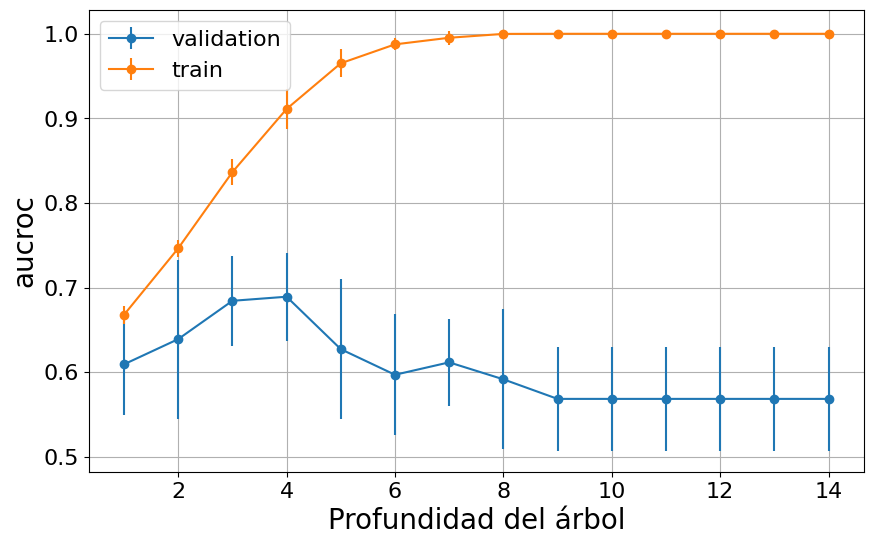
\includegraphics[width=0.49\textwidth]{/files/src/.media/decisionTreeComplexity.png}
    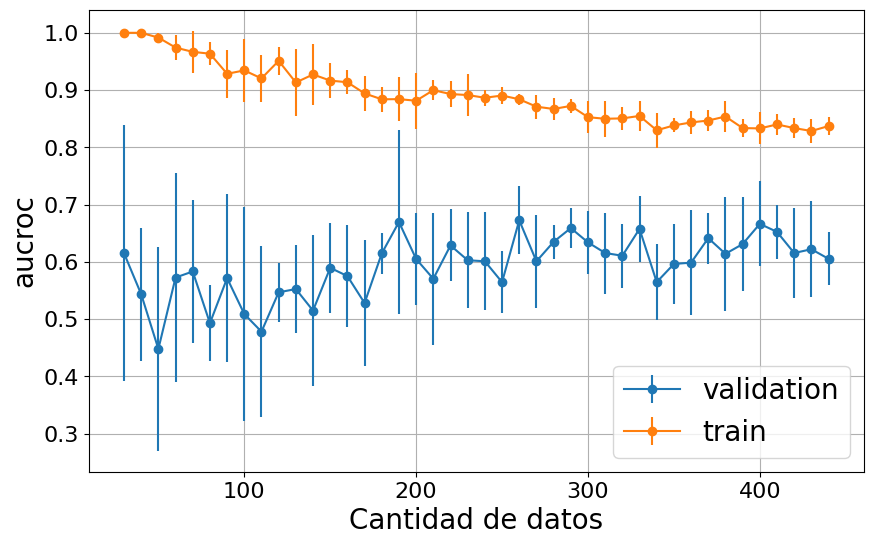
\includegraphics[width=0.49\textwidth]{/files/src/.media/decisionTreeLearning.png}
    \caption{Clasificador \textit{decision tree}. Izquierda: Curvas de complejidad mostrando la variación del \textit{aucroc} a medida que se aumenta la profundidad máxima. Derecha: Curvas de aprendizaje mostrando la variación del \textit{aucroc} a medida que se aumenta el tamaño del dataset.}
    \label{decisionTreeComplexity}
\end{figure}

Con respecto a la varianza, podemos observar que el rendimiento de los modelos varía considerablemente según el dataset utilizado en entrenamiento. Esto puede apreciarse en las barras de error\footnote{Estas provienen de las mediciones de AUC ROC para cada fold de validación.}, donde en algunos casos como para \textit{altura máxima} = 2 y 5, hubo una diferencia de performance en más de un $10\%$. A su vez, puede verse cómo se van separando ambas curvas a medida que aumenta la profundidad máxima. Es decir, la performance del modelo en entrenamiento aumenta al hacer \textit{overfitting} mientras que en validación decrece. Esto muestra que la varianza del clasificador crece junto con la profundidad máxima, ya que el modelo se acopla cada vez más al dataset.

Por otro lado, todos los resultados del algoritmo en validación se encuentran con un AUC ROC por debajo de $0.75$, y con media aproximadamente en $0.6$, con lo cual parecería tener poca capacidad predictiva. En ese sentido, sin importar el valor del hiperparámentro parecería ser un algoritmo incapaz de acercarse a la distribución subyacente de los datos, produciendo \textit{underfitting} y presentando un sesgo alto.

% 2. Graficar curvas de aprendizaje para cada modelo. En base a estas curvas, sacar conclusiones sobre si los algoritmos parecen haber alcanzado su límite, o bien si aumentar la cantidad de datos debería ayudar.

Variando la cantidad de datos de entrenamiento en el rango $[30, n]$ con un step de $10$, siendo $n$ la cantidad total de instancias, obtuvimos las curvas de aprendizaje de la Figura \ref{decisionTreeLearning}. De ellas podemos observar que, con pocos datos ($< 150$ instancias), el modelo parecería funcionar igual, a veces hasta peor, que un clasificador aleatorio, con un AUC ROC en promediado rondando el $0.5$. Al aumentar la cantidad de datos, puede observarse como ambas curvas se van acercando entre sí, para luego estabilizarse en los valores $0.85$ para el set de entrenamiento y $0.6$ para el de validación. Esto indica que el algoritmo, sin importar cuánto aumentemos el tamaño del set de entrenamiento, parecería haber encontrado su límite de aprendizaje.

\subsection{Linear discriminant analysis}

En el caso de este clasificador, no tiene sentido hablar de curvas complejidad al no poseer un hiperparámentro que la regule. Por otro lado, trazamos las curvas de aprendizaje expresadas en la Figura \ref{LDALearning}, variando la cantidad de datos con los que fue entrenado. 

En ella, podemos apreciar que el modelo posee un sesgo bajo, teniendo en cuenta que su performance se estabiliza cerca del valor $0.8693$ al contar con $> 200$ datos. También, se puede ver que a partir de ese tamaño de dataset el modelo deja de aprender sobre el dominio del problema y mantiene una performance estable, con lo cual contar con más datos no lo beneficiaría significativamente. En particular, el mejor valor de \textit{auc roc} obtenido fue de $0.88$ para $250$ datos\footnote{Dado que en la construcción de las curvas de aprendizaje en cada iteración se aumenta la cantidad de datos de entrenamiento, no nos pareció correcto resetear el \textit{random state} en el proceso de validación cruzada. Luego, los resultados difieren un poco con respecto a los obtenidos durante la búsqueda aleatoria.}.

Por último, también se puede apreciar que al aumentar la cantidad de datos, las barras de error se van achicando, con lo cual la varianza del modelo diminuye. En general, el modelo parecería poseer baja varianza para una cantidad de datos $> 200$. De manera tentativa, calculamos el promedio de las deviaciones estándar a partir de este tamaño de dataset, y su valor fue aproximadamente $0.05$.

\begin{figure}[!htbp]
    \centering
    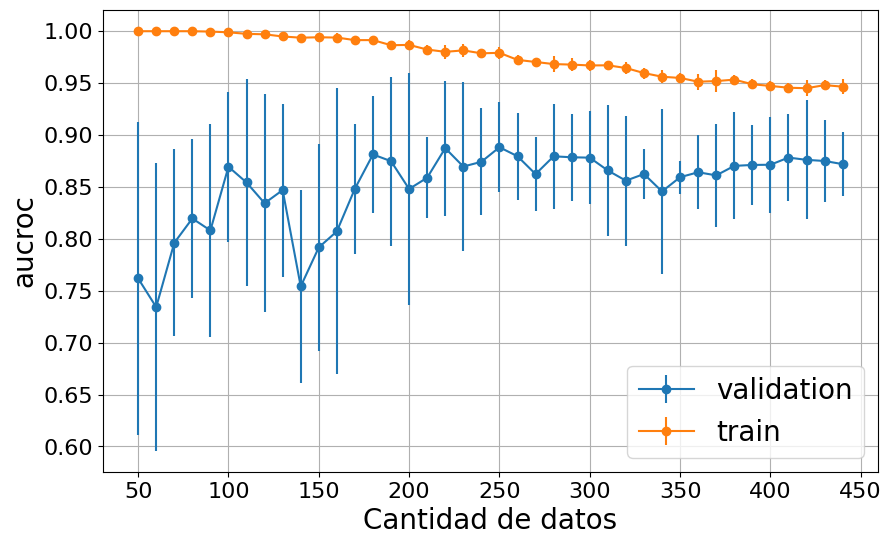
\includegraphics[width=0.49\textwidth]{/files/src/.media/LDALearning.png}
    \caption{Clasificador \textit{Linear Discriminant Analisis}. Curvas de aprendizaje mostrando la variación del \textit{aucroc} en datos de entrenamiento y validación a medida que se aumenta la cantidad de datos. Las líneas verticales denotan la varianza para cada tamaño de dataset.}
    \label{LDALearning}
\end{figure}

\subsection{Support vector machines}

Basándonos en la mejor configuración de hiperparámetros hallada en el ejercicio 3, procedimos a realizar una curva de complejidad variando el C y analizando como varía la performance del SVM. 

El hiperparámetro C permite generar un control de la penalización por errores de clasificación. Un valor mayor de C significa que el modelo penalizará más los errores de clasificación lo cual implica que buscará un hiperplano de separación que clasifique correctamente la mayor cantidad posible de ejemplos de entrenamiento. Por otro lado, un valor de C menor permite que el modelo tolere más errores de clasificación y puede resultar en un hiperplano de separación más general, incluso si esto significa clasificar incorrectamente algunos ejemplos de entrenamiento.

\begin{figure}[!htbp] 
    \centering
    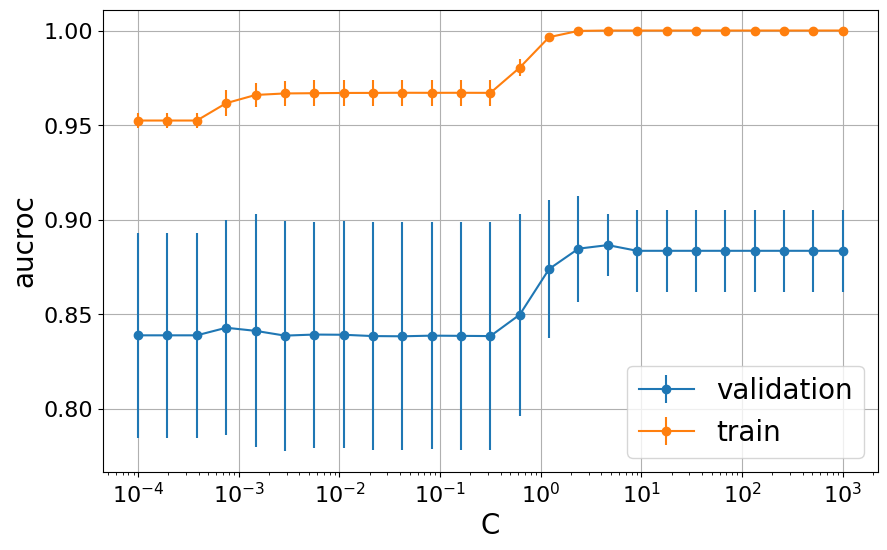
\includegraphics[width=0.49\textwidth]{/files/src/.media/SVMComplexity.png}
    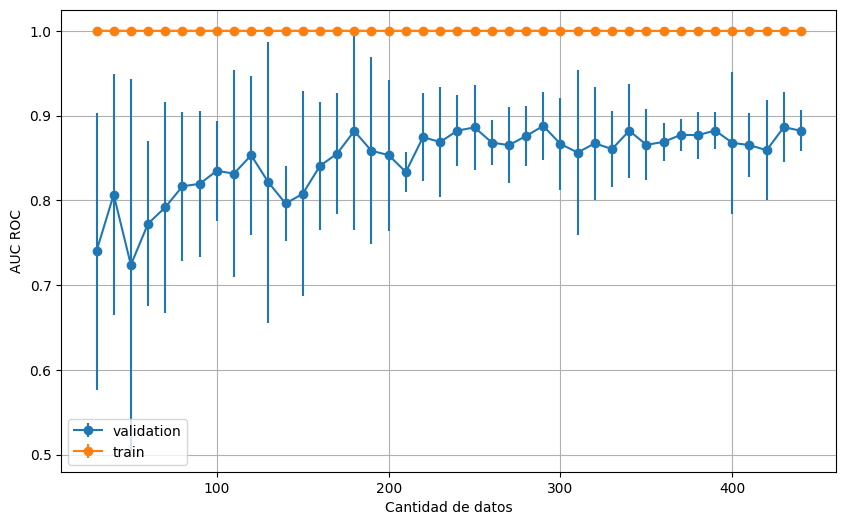
\includegraphics[width=0.49\textwidth]{/files/src/.media/SVMLearning.png}
    \caption{Clasificador \textit{SVM}. Izquierda: Curvas de complejidad mostrando la variación del \textit{aucroc} a medida que se aumenta \textit{C}. Derecha: Curvas de aprendizaje mostrando la variación del \textit{aucroc} a medida que se aumenta el tamaño del dataset.}
    \label{SVM}
\end{figure}

Como se puede ver en la Figura \ref{SVM}, el hiperparámetro C afecta a la performance del algoritmo, aunque no de forma considerable. En base a lo observado el algoritmo es bastante bueno para modelar el problema, ya que sin importar el C elegido la media de AUCROC es bastante alta. En cambio un C incorrecto genera que la varianza de la performance de los folds sea alta, por lo que elegir el C correcto pareciera tener un mayor impacto en la estabilidad del modelo que en la performance.

La curva de aprendizaje en la Figura \ref{SVM} nos permite determinar que la cantidad de datos es suficiente para armar un modelo decente de SVM, ya que a partir de 250 datos, pareciera mantener una performance constante sin denotar una clara tendencia creciente. Algo a destacar es que, a diferencia de árboles de decisión, las barras de error incluso considerando casi todos los datos, siguen mostrando una gran variabilidad en tamaño, lo cual denota una posible inestabilidad del algoritmo.

\subsection{Random Forest}

Primero realizamos un Random Search para encontrar hiperparámetros decentes para Criterion y para maxdepth. Luego realizamos una curva de complejidad variando el maxfeatures, que nos serviría para entender como afecta este hiperparámetro a la performance del Algoritmo. 

\begin{figure}[!htbp]
    \centering
    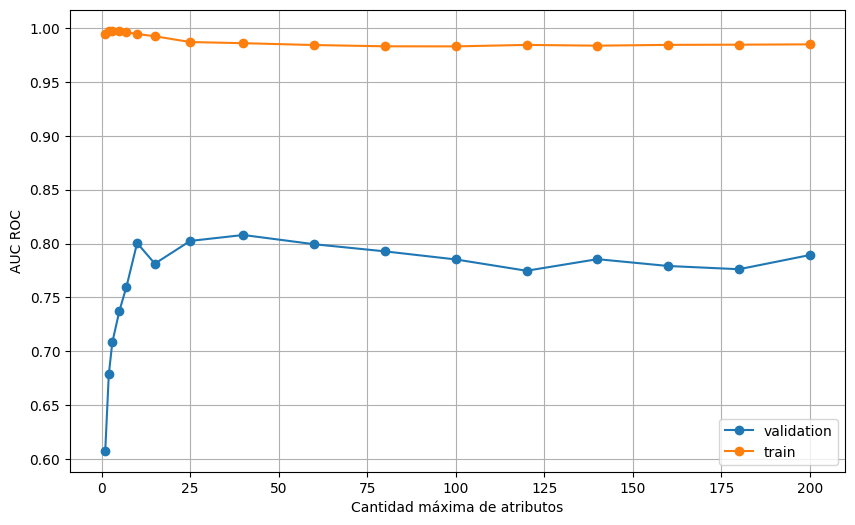
\includegraphics[width=0.49\textwidth]{/files/src/.media/randomForestComplejidad.png}
    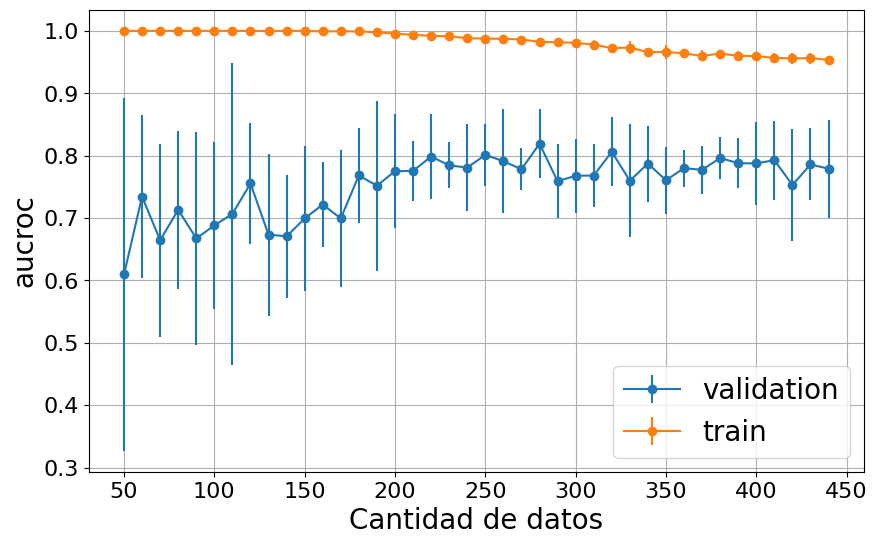
\includegraphics[width=0.49\textwidth]{/files/src/.media/randomForestAprendizaje.png}
    \caption{Clasificador \textit{Random Forest}. Izquierda: Curvas de complejidad mostrando la variación del \textit{aucroc} a medida que se aumenta \textit{maxFeatures}. Derecha: Curvas de aprendizaje mostrando la variación del \textit{aucroc} a medida que se aumenta el tamaño del dataset.}
    \label{RF}
\end{figure}

La figura \ref{RF} nos muestra algo que tiene sentido que es que cuando maxfeatures es muy bajo genera un impacto negativo en la performance del algoritmo. Esto tiene sentido ya que maxfeatures representa la cantidad de atributos tomados de manera aleatoria que cada decision tree que compone el forest va a considerar en cada paso del algoritmo. Es lógico que si considerás muy pocos atributos para realizar los cortes no encuentres buenas opciones y por lo tanto tengas un modelo defectuoso.

Por otro lado, la figura nos muestra otro resultado que no es tan intuitivo, que es que maxfeatures rápidamente alcanza su límite en el impacto en la performance y luego a medida que sigue aumentando, incluso pareciera decrecer ligeramente. Este resultado es particularmente atractivo, ya que si bien a medida que crece no mejora considerablemente la performance, si afecta directamente el costo computacional. 

La posible explicación para porque puede ser contraproducente tener un maxfeatures muy alto es que mientras más atributos se consideren en cada corte, menos variabilidad vamos a encontrar entre los árboles que componen el bosque. Es decir, los árboles resultantes van a ser más parecidos entre sí, lo cual genera un \textit{overfitting} de los datos.  

Concluimos que tiene sentido tomar logaritmo o sqrt de la cantidad de atributos de los datos para mantener maxfeatures dependiente de la cantidad de atributos, pero que sea realativamente bajo para tener una buena performance y minimizar la complejidad computacional. 

Por otro lado, graficamos una curva de aprendizaje (Figura \ref{RF}) para determinar si sería útil o no conseguir más datos. Lo que observamos a partir de la figura, es que a partir de 200 datos la performance del algoritmo parece mantenerse constante sin notar una tendencia alcista. Concluimos que la cantidad de datos provista es suficiente como para generar un modelo decente basado en random forest. 

Algo interesante a destacar de la curva de aprendizaje del random forest es que las barras de error son consistentemente pequeñas a medida que se aumentan los datos. 